\section{Objetivos}
\begin{itemize}
    \item Medir el campo eléctrico de un condensador de placas paralelas, utilizando un medidor de campo eléctrico para determinar cómo varía el campo en función de diferentes configuraciones y distancias entre las placas.
    \item Identificar y comprender las diferencias y similitudes entre la conexión de condensadores en serie y en paralelo, y cómo estas configuraciones afectan las propiedades eléctricas del sistema.
\end{itemize}

\section{Marco Teórico}
El potencial eléctrico se define como la energía potencial por unidad de carga de prueba, expresada matemáticamente como $\Delta V = \frac{\Delta U}{q_0}$, donde $\Delta U$ es la variación de la energía potencial y $q_0$ es la carga de prueba. Esta definición establece que el potencial eléctrico es un escalar y se mide en voltios (V), donde $1 V = 1 \frac{J}{C}$.

El campo eléctrico entre dos placas paralelas conductoras es de especial interés. Cuando las placas se cargan, el campo eléctrico entre ellas es casi uniforme y está casi completamente localizado entre las placas. La magnitud de este campo eléctrico, $E$, puede ser derivada aplicando el principio de superposición y se calcula mediante la relación $E = \frac{\sigma}{\epsilon_0}$, donde $\sigma$ es la densidad superficial de carga y $\epsilon_0$ es la permitividad del vacío.

Para placas paralelas con una separación $d$ pequeña en comparación con sus dimensiones, la diferencia de potencial entre las placas puede calcularse como $V_{ab} = E d = \frac{q d}{\epsilon_0 A}$, mostrando cómo el campo eléctrico se relaciona directamente con la carga y la geometría de las placas.

Además, se discutirá la conexión de condensadores en serie y paralelo:
\begin{itemize}
    \item En serie, los condensadores comparten la misma carga y la tensión total se distribuye entre ellos según sus capacitancias inversas.
    \item En paralelo, todos los condensadores experimentan la misma diferencia de potencial y las cargas se suman, aumentando la capacitancia total.
\end{itemize}

Estos principios son fundamentales para entender cómo se distribuyen y manejan las cargas eléctricas en sistemas más complejos y son esenciales para diseñar circuitos eléctricos eficientes y efectivos.

\section{Análisis y discusión: Montaje 1}

\subsection{Montar capacitor}
\textbf{Montar el capacitor de placas paralelas, como se muestra en la Figura 1, deje un
espacio entre las placas de $d = 6.5cm$.}

\subsection{Verificar Medidor}
\textbf{Verificar que el medidor de campo eléctrico marca cero cuando no se aplica un
voltaje.}

\subsection{Campo eléctrico entre placas paralelas}
\textbf{Reportar el campo eléctrico entre las placas paralelas para los siguientes voltajes.}

\begin{figure}[H]
    \centering
    \begin{subfigure}[b]{\textwidth}
        \centering
        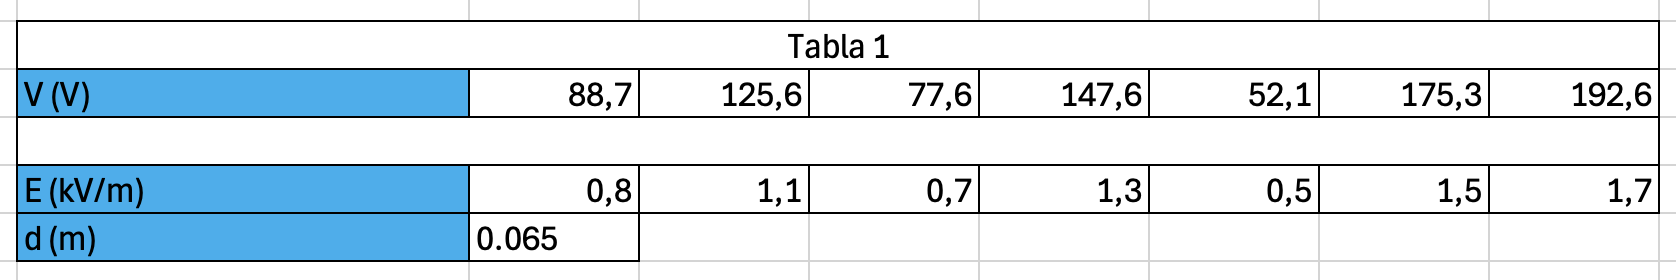
\includegraphics[width=\textwidth]{Figures/1. Content/tablaCampoVSV.png}
        \caption{Tabla Campo eléctrico $E$ y $V$}
        \label{fig: tabla Campo vs V}
    \end{subfigure}
    \hfill
\end{figure}


\subsection{Graficar $\Delta V$ vs $E$}

\begin{figure}[H]
    \centering
    \begin{subfigure}[b]{\textwidth}
        \centering
        \includegraphics[width=\textwidth]{Figures/1. Content/CampoVSV.png}
        \caption{Campo eléctrico $E$ y $V$}
        \label{fig: Campo vs V}
    \end{subfigure}
    \hfill
\end{figure}

\subsection{¿Qué tipo de relación se encuentra en la gráfica del numeral 3.4?}
La gráfica de $V$ (Voltaje) versus $E$ (Campo eléctrico) muestra una relación lineal, como indica la ecuación de la línea de mejor ajuste $y = 0.0084x + 0.0518$ y un coeficiente de determinación ($R^2$) muy cercano a 1 ($R^2 = 0.9985$). Esto implica que el campo eléctrico entre las placas de un capacitor aumenta proporcionalmente con el aumento del voltaje aplicado, lo cual es consistente con la teoría de que $E = \frac{V}{d}$ para un capacitor de placas paralelas con distancia $d$ constante entre las placas.

\subsection{¿Qué significado físico tiene la pendiente?}
La pendiente de la recta en la gráfica de $V$ vs $E$, que es aproximadamente $0.0084$ kV/m por V, representa el cambio en el campo eléctrico por unidad de cambio en el voltaje aplicado, es decir, $\frac{1}{d}$, donde $d$ es la separación entre las placas del capacitor. Este valor es teóricamente igual a $\frac{1}{d}$, asumiendo que la distancia entre las placas no cambia. Esto valida la relación directa entre el campo eléctrico y el voltaje en un capacitor de placas paralelas, donde $E = \frac{V}{d}$.

\subsection{¿Qué valor se espera encontrar en la pendiente del numeral 3.4?}
Teóricamente, se espera que la pendiente de la gráfica $V$ vs $E$ sea $\frac{1}{d}$. Dado que la distancia entre las placas $d$ es constante y conocida (0.065 m en este caso), la pendiente esperada es aproximadamente $\frac{1}{0.065}$ m\(^{-1}\) o aproximadamente $15.38$ kV/m por V. La discrepancia entre este valor teórico y el valor experimental observado ($0.0084$ kV/m por V) puede deberse a errores experimentales o suposiciones en la teoría, como la uniformidad del campo entre las placas o la precisión en la medición del voltaje y la distancia.

\section{Procedimiento Experimental y Resultados: Montaje 2}

\subsection{Variar separación de entre placas}
\textbf{Fijar el voltaje en $\Delta V = 100V$, variar la separación entre las placas de acuerdo con
la siguiente tabla y reportar el valor medido de $E$.}
\begin{figure}[H]
    \centering
    \begin{subfigure}[b]{\textwidth}
        \centering
        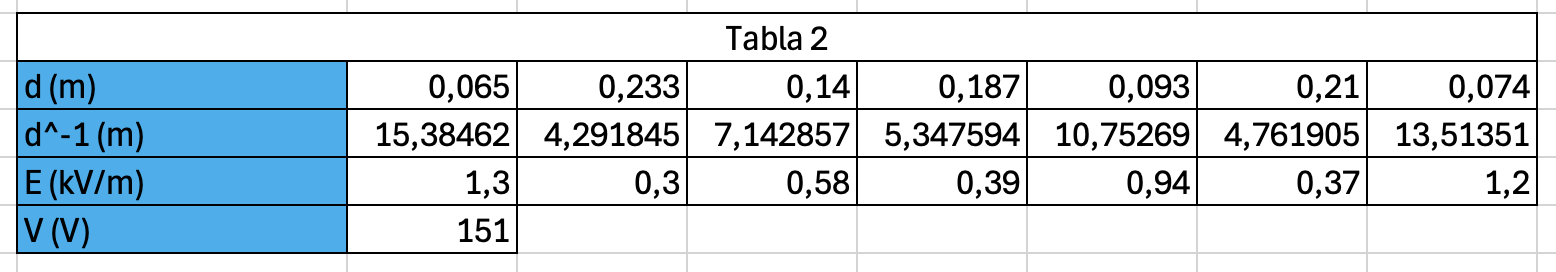
\includegraphics[width=\textwidth]{Figures/1. Content/tablaCampoVSd1.png}
        \caption{Tabla Campo eléctrico $E$ y $d^{-1}$}
        \label{fig: tabla Campo vs d^-1}
    \end{subfigure}
    \hfill
\end{figure}

\subsection{Graficar $E$ vs $d^{-1}$}

\begin{figure}[H]
    \centering
    \begin{subfigure}[b]{\textwidth}
        \centering
        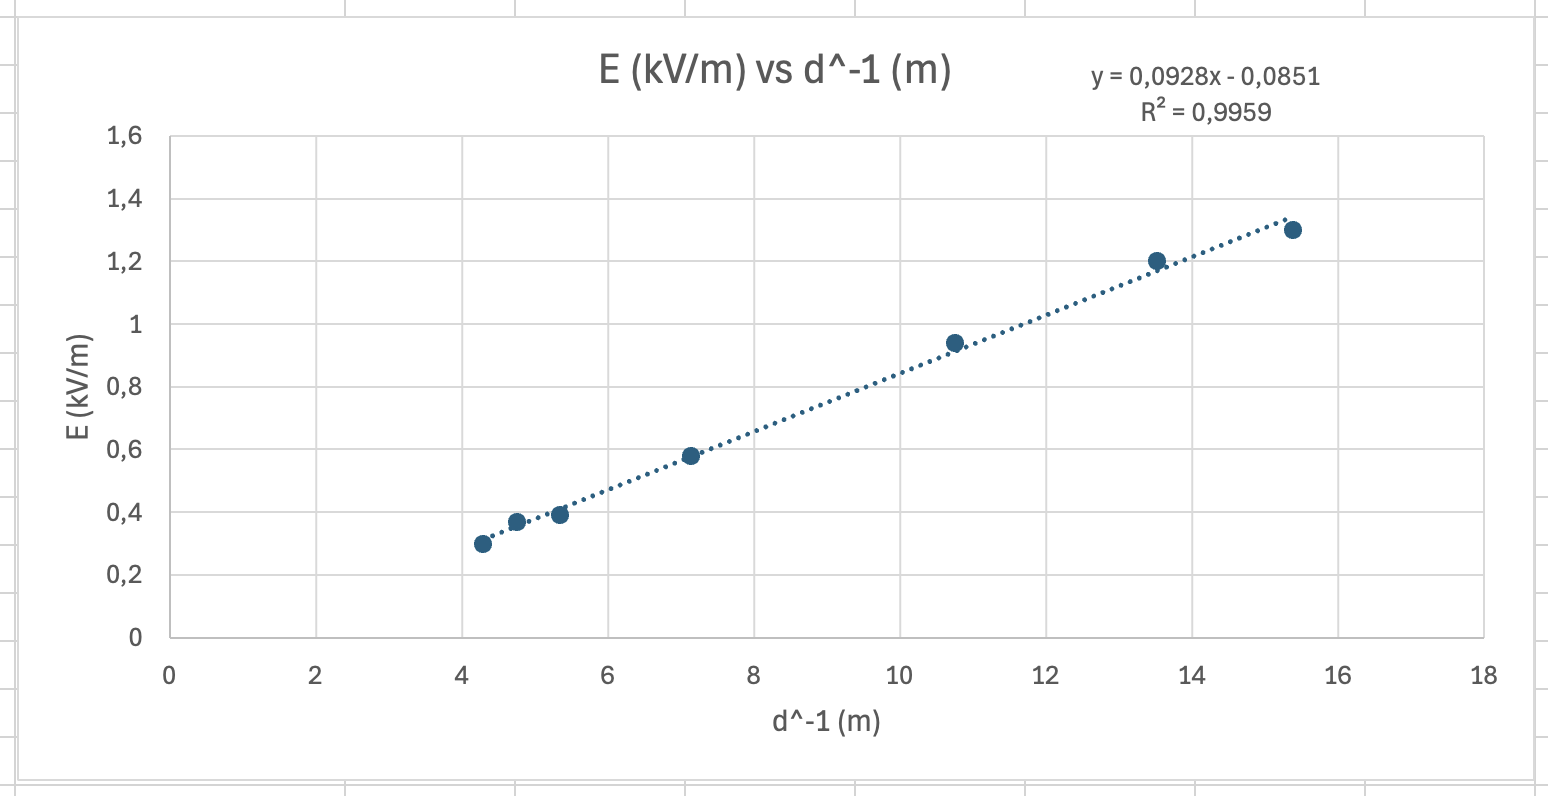
\includegraphics[width=0.8\textwidth]{Figures/1. Content/campoVSd1.png}
        \caption{Campo eléctrico $E$ vs $d^{-1}$}
        \label{fig: Campo vs d^-2}
    \end{subfigure}
    \hfill
\end{figure}

\subsection{¿Qué tipo de relación se encuentra en la gráfica del literal 4.2?}
La gráfica que relaciona el campo eléctrico \( E \) con el inverso de la distancia \( d^{-1} \) entre las placas muestra una dependencia lineal, evidenciada por la ecuación de la línea ajustada \( y = 0.0928x - 0.0851 \) y un coeficiente de correlación muy elevado (\( R^2 = 0.9959 \)). Esto demuestra que el campo eléctrico es proporcional al inverso de la distancia entre las placas, como predice la fórmula \( E = \frac{V}{d} \), indicando que a menor distancia, mayor es el campo eléctrico generado para un voltaje constante.

\section{Procedimiento Experimental y Resultados: Montaje 3}

\subsection{Valores de montaje de capacitancias}

\begin{figure}[H]
    \centering
    \begin{subfigure}[b]{\textwidth}
        \centering
        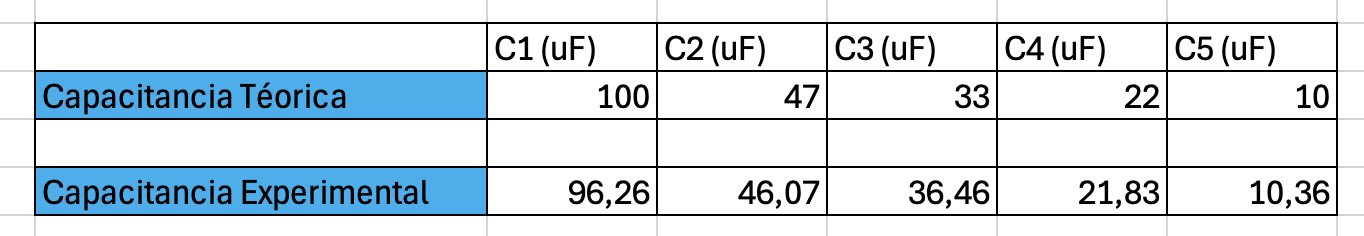
\includegraphics[width=0.8\textwidth]{Figures/1. Content/MontajeCapacitancias.png}
        \caption{Valores de montaje de capacitancias}
        \label{fig: Valores de montaje de capacitancias}
    \end{subfigure}
    \hfill
\end{figure}

\subsection{Montaje de capacitancias en Serie}

\begin{figure}[H]
    \centering
    \begin{subfigure}[b]{\textwidth}
        \centering
        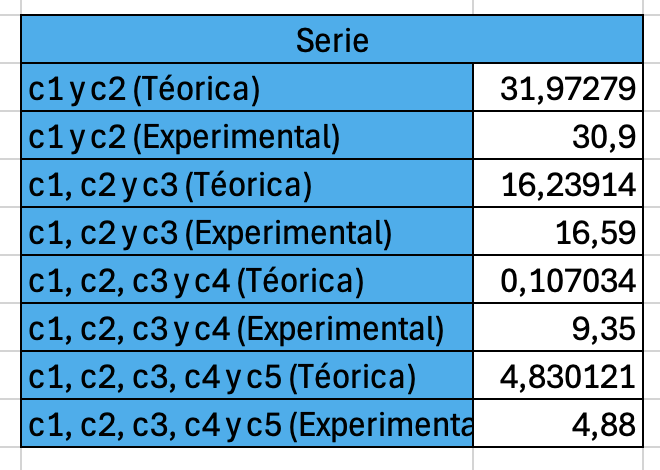
\includegraphics[width=0.8\textwidth]{Figures/1. Content/MontajeCapacitanciasSerie.png}
        \caption{Valores de Montaje de capacitancias en Serie}
        \label{fig: Montaje de capacitancias en Serie}
    \end{subfigure}
    \hfill
\end{figure}

\subsection{Montaje de capacitancias en Paralelo}

\begin{figure}[H]
    \centering
    \begin{subfigure}[b]{\textwidth}
        \centering
        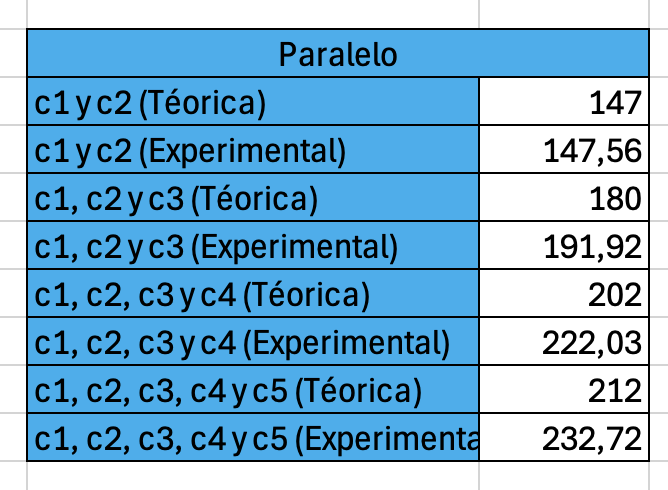
\includegraphics[width=0.8\textwidth]{Figures/1. Content/MontajeCapacitanciasParalelo.png}
        \caption{Valores de Montaje de capacitancias en Paralelo}
        \label{fig: Montaje de capacitancias en Paralelo}
    \end{subfigure}
    \hfill
\end{figure}


\subsection{Montaje de capacitancias Extras}

\begin{figure}[H]
    \centering
    \begin{subfigure}[b]{\textwidth}
        \centering
        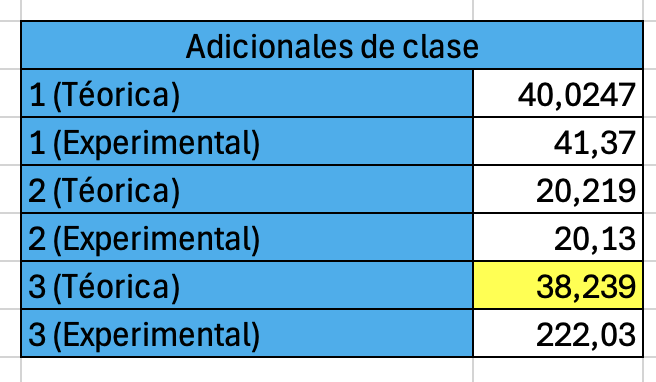
\includegraphics[width=0.8\textwidth]{Figures/1. Content/MontajeCapacitanciasExtra.png}
        \caption{Valores de Montaje de capacitancias Extras}
        \label{fig: Montaje de capacitancias Extras}
    \end{subfigure}
    \hfill
\end{figure}

\subsection{Análisis de Capacitores en Serie}
\textbf{¿Se puede afirmar que para un sistema de capacitores en serie el capacitor
equivalente es menor a la menor de las capacitancias?}
Se puede afirmar que para un sistema de capacitores en serie, el capacitor equivalente siempre es menor que la menor de las capacitancias individuales. Esto se debe a que la capacitancia equivalente para capacitores en serie se calcula como:

\[
\frac{1}{C_{eq}} = \frac{1}{C_1} + \frac{1}{C_2} + \cdots + \frac{1}{C_n}
\]

donde \( C_{eq} \) es la capacitancia equivalente y \( C_i \) son las capacitancias individuales. Esta relación asegura que \( C_{eq} \) sea menor que la menor capacitancia individual, como lo corroboran los resultados experimentales.

\subsection{Análisis de Capacitores en Paralelo}
\textbf{¿Se puede afirmar que para un sistema de capacitores en paralelo el capacitor
equivalente es mayor a la mayor de las capacitancias?}
Para capacitores en paralelo, se puede afirmar que el capacitor equivalente siempre es mayor que la mayor de las capacitancias individuales. La capacitancia equivalente se determina sumando las capacitancias individuales:

\[
C_{eq} = C_1 + C_2 + \cdots + C_n
\]

Este cálculo produce una capacitancia equivalente \( C_{eq} \) que supera cualquier capacitancia individual, confirmado igualmente por los datos experimentales.

\section{Causas de Error}
Las principales causas de error en este experimento podrían incluir:
\begin{itemize}
    \item Inexactitudes en la calibración del voltímetro y del medidor de campo eléctrico, que podrían haber afectado la precisión de las mediciones de voltaje y campo eléctrico.
    \item Variaciones en la separación real entre las placas comparada con la separación medida, afectando la relación calculada del campo eléctrico.
    \item Influencias de campos electromagnéticos externos, especialmente si el laboratorio no está adecuadamente aislado de fuentes de interferencia.
    \item Errores en la conexión y configuración de los capacitores, especialmente en las configuraciones de serie y paralelo, que podrían afectar las mediciones de capacitancia.
    \item Humedad ambiental que podría haber influido en las propiedades dieléctricas de las placas, alterando los valores esperados del campo eléctrico y las capacitancias.
\end{itemize}

\section{Conclusiones}
A partir del experimento realizado, se pueden extraer las siguientes conclusiones:
\begin{itemize}
    \item Los resultados confirmaron la teoría de que el campo eléctrico entre dos placas paralelas es directamente proporcional al voltaje aplicado y varía inversamente con la distancia entre las placas.
    \item Se verificó que para capacitores en serie, el capacitor equivalente es siempre menor que la menor capacitancia individual de los capacitores involucrados. Esto es consistente con la teoría y se observó en todas las configuraciones de serie experimentadas.
    \item Para los capacitores en paralelo, se confirmó que el capacitor equivalente siempre es mayor que la mayor capacitancia individual. Esto fue apoyado por las mediciones experimentales, donde las capacitancias equivalentes excedieron la mayor capacitancia individual en cada configuración de paralelo probada.
    \item Las discrepancias observadas entre los valores teóricos y experimentales de las capacitancias sugieren la presencia de factores perturbadores no contemplados en el análisis inicial, destacando la importancia de considerar variables ambientales y técnicas de medición en la interpretación de resultados experimentales.
\end{itemize}